\section{Introduction}\label{sec:intro}

Pattern matching in distributed environments is
generally considered a challenging but important task for applications
relevant to machine-to-machine (M2M) systems. In such
settings where a large amount of local machines are involved in computation and storage, a primary goal is often to minimize the amount of communication
needed to compute the answer.  This paper aims at advancing the
current state-of-the-art on distributed pattern matching from
`single reference pattern' to `multiple reference patterns', and proposes a general framework
to handle both $k$ nearest and farthest neighbor search of the multiple reference pattern set, while
significantly reducing the communication cost, mainly the bandwidth consumption.

Consider a first scenario in which, through sensor data in a specific
area, a scientist detects some unusual and potentially dangerous event
(e.g., the dramatic oscillation of CO2 level), and wants to learn
quickly whether a similar event has happened at other places. To do
so, it is required to use the signal obtained by multiple sensors in
one area to match sensor signals produced in the other areas.  A
second scenario assumes a distributed database of historical sensor
readings such as the past 50 years' temperature information for many
locations.  Researchers might want to specify a set of time series
that they identify with a certain known event (e.g., El Ni\~{n}o,
solar activity, or the increased spread of a pest-borne disease) and
query the distributed database to determine the wheres and whens of
the most similar patterns.  A third scenario assumes that we are
monitoring certain environmental levels at many locations, and we
would like to issue a warning whenever a location's pattern of recent
levels deviates significantly, but perhaps subtly, from the recent
patterns at a set of reference locations, because it might indicate an
abnormal environmental event is happening at that location (e.g.,
hazardous material being improperly transported).

% To accomplish the above task efficiently, one common criteria is minimize the transmission costs between query server and local machines to save bandwidth, energy, and time. have we have a potentially dangerous person to monitor. Say, we want to prevent this person from getting onto any plane. However, what we have are some photos of this person wearing a variety of clothes, while some photos might be clearer than others. An matching  system deployed in security gates of airports would have to take multiple photos as an input, and raise a flag when there is a plausible match. Consider a second scenario, where the photo of every employee in the company are available, and our goal is to design a surveillance system that would issue an warning whenever somebody who does not belong to this company enters any company property. The third scenario in an M2M environment is that assuming we have gathered signals from $M$ different sensors in close-by locations before certain disaster, e.g., tsunami, and would like to design a forecasting system for similar event. In this case, the system has to take the $m$ different time series into account while performing matching. 

Designing a general framework that can handle the above scenarios
requires addressing several challenges. First, the query to be matched
may consist of multiple patterns, in order to provide a more robust
reference set beyond what any one pattern might provide.  For
example, there may be more than one ``signature'' pattern for an event
or more than one nearby sensor monitoring an event.  The multiple patterns
in a single query may be highly correlated, such as when collected by
nearby sensors (1$^{st}$ and 2$^{nd}$ scenarios), or only moderately
correlated, such as when collected from a set of reference locations
(3$^{rd}$ scenario).  Second, the query to be matched is often a
one-time (i.e., snapshot) query, either posed as an ad hoc query
(1$^{st}$ and 2$^{nd}$ scenarios) or as a continuous sequence of
queries such that recent readings determine the next query in the
sequence (3$^{rd}$ scenario).  Third, we need to handle not only
\emph{similarity} (1$^{st}$ and 2$^{nd}$ scenarios) but also \emph{dissimilarity}
(3$^{rd}$ scenario) search.  Fourth, we seek the $k$ most similar (or
$k$ most dissimilar) neighbors from across a potentially large
collection of \emph{distributed} data sources.  Finally, because in
many situations there are bandwidth limitations and concerns of energy
consumption as well as cost during communication, it is usually
critical to design an approach that requires as little communication
between machines as possible. To be more precise, our goal is to reduce
the bandwidth consumption while not missing any $k$ most similar/dissimilar neighbors.

\begin{figure}[tbp]
\centering
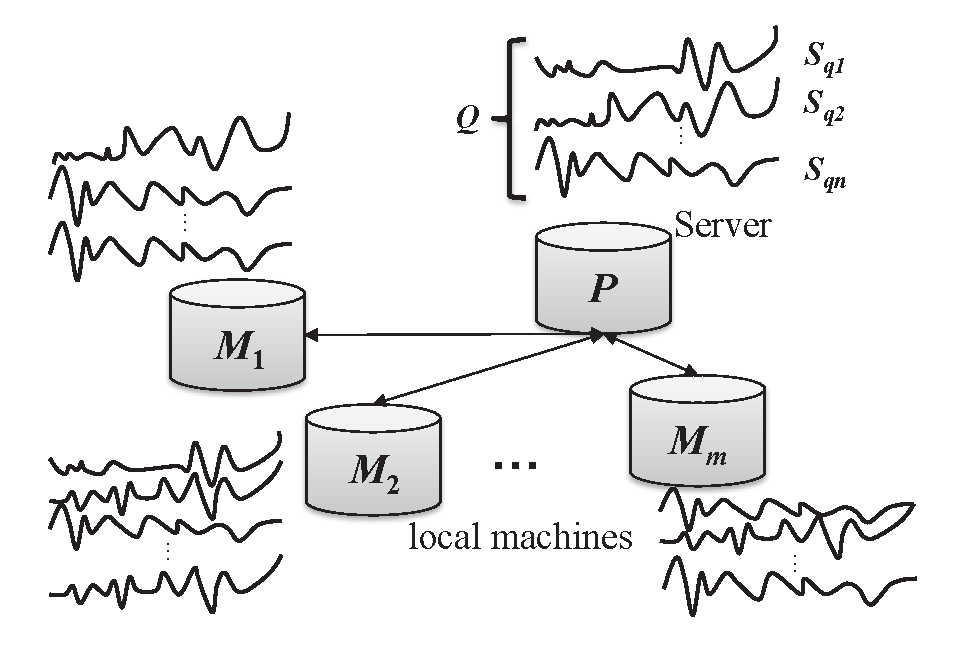
\includegraphics[width=0.6\linewidth]{system-model.eps}
\vspace{-0.1in}
\caption{The system model}
\label{fig:system-model}
\vspace{-0.2in}
\end{figure}

To address the above challenges, we propose a new framework that,
given multiple reference patterns, allows us to find their exact $k$-nearest (most similar) and $k$-farthest (most dissimilar) neighbors, denoted as $k$NN and $k$FN, in a distributed environment where bandwidth is limited. In M2M applications such as the aforementioned three scenarios, a huge amount of measurement readings over a period of time are collected. Therefore the multiple reference patterns to be dealt with in this paper are mainly multiple time series. The system diagram can be seen in Fig.~\ref{fig:system-model}, where there are $m$ distributed machines, each monitoring one or more series of measurement readings, and a server orchestrating
the processing of $k$NN and $k$FN discoveries. Given a set $Q$ of multiple time series patterns as the query at the server, the goal is to find a set of $k$ time series among all $m$ local machines with the highest similarity (or
dissimilarity) to the query.  Our primary cost metric is the total
number of bytes exchanged between the server and the local machines to
answer the query. We do not explicitly model the small cost that may
sometimes be required to assemble the query at the server such as in the 3$^{rd}$
scenario.  Also, while we do not explicitly model response time, our
solutions are highly parallel and fast.

Prior work has considered $k$NN search for the system model in Fig.~\ref{fig:system-model},
but restricted to a single reference pattern (i.e., $|Q|=1$)~\cite{PAP01DPS,Yeh:2008:LLD}.
In a naive solution the server sends the query to each local machine, each local machine computes
the $k$NN to the query from among the locally maintained measurement readings and sends
them back to the server, and finally the server determines the overall $k$NN solution
from among the results received.  This solution, called \textit{Concurrent Processing 
(CP)}~\cite{PAP01DPS}, incurs a high bandwidth cost because 
each of the $m$ machines sends back $k$ results, out of which only $k$ are in the overall
solution.  To address this, Papadopoulos and Manolopoulos~\cite{PAP01DPS} 
proposed the \textit{Probabilistic Processing method (PRP)}, which reduces the amount of data 
required to be transmitted back to the server from the local machines.
To further reduce bandwidth consumption, our earlier work~\cite{Yeh:2008:LLD} proposed
\LeeWave{}, which leverages the multi-resolution property of the Haar wavelet 
transformation of time series. However, none of this prior work considered multiple 
reference patterns or $k$FN search, and straightforward generalizations of \LeeWave{}
produce incorrect results (as we will show in Section~\ref{subsec:limitations}).

Our framework, called \MSWave{}, 
is designed based on the following insights. First, to
handle multiple reference patterns as queries, we propose three distance measurements, 
namely \emph{single-linkage distance}, \emph{average-linkage
distance}, and \emph{complete-linkage distance}, which report the
shortest, average, and largest distances among all the distances of a
candidate time series to each reference pattern in the query set. The above
three distance measures are analogous to the single-link, average-link, and
complete-link clustering models. Second, based on the characteristics
of the Haar wavelet transform, \MSWave{} pre-processes each series of measurement readings by
decomposing it into a multi-resolution representation. Instead of
sending the whole query set $Q$ to the local machines, the server
iteratively sends information on each query in $Q$ in a level-wise manner starting
with the coarsest resolution (fewest bytes sent) and continuing with increasingly finer 
resolutions (more bytes sent).
We further derive and
maintain certain similarity range bounds for each of the three
distance measurements, such that the upper and lower bounds can be incrementally
updated at each iteration/level.  More importantly, we prove that these similarity range
narrow as we move from one wavelet coefficients level to the next,
enabling effective pruning of the candidate time series that reduces bandwidth consumption
without causing any false dismissal.  Although prior work has proposed
wavelet level-wise pruning strategies~\cite{Yeh:2008:LLD, Kashyap:2011:SKS},
we not only generalize it to multiple reference patterns but also further reduce
bandwidth by shifting the similarity bounds calculations from the server
to the local machines.  
%This enables tighter bounds (better pruning) as well as 
%a different communication strategy that saves even more bandwidth.

%We present an analysis demonstrating the significant bandwidth savings from
%shifting the similarity bounds calculations to the local machines.
We conduct extensive experiments using both real and synthetic data. The
results show that our solution significantly outperforms the
competitive approaches in total bandwidth consumption in a variety of
different setups for searching both $k$NN and $k$FN.

Our main contributions can be summarized as follows:
\begin{itemize}
\item
We present \MSWave{}, a general communication-efficient framework to
identify both $k$NN and $k$FN instances given multiple time series reference patterns in
a distributed environment. To our knowledge, this is the
first solution proposed for such purpose.
\item
Methodology-wise, we propose to use average, closest, and
furthest neighbor distance to process multiple query (dis)similarity.
We then take advantage of the multiple-resolution property
of wavelet coefficients, and then for each distance measurement we derive
upper and lower bounds of the similarity between each candidate time series
to the query set. Such bounds can be exploited
to prune candidates for more efficient search without compromising correctness. Moreover,
in further contrast to prior approaches, we propose to shift the
bounds computation from the server to the local machines to further reduce the bandwidth
consumption.
\item
We conduct theoretical analysis and proofs to validate several
of our arguments, including the infeasibility/feasibility of the
existing/proposed approaches, and derive the equation to represent the
bandwidth savings from shifting the bounds computations to the local machines.
Finally, we conduct extensive experiments that demonstrate \MSWave{}'s 
significant bandwidth savings.
\end{itemize}

